\documentclass{mwart}
\usepackage{geometry}
\usepackage{amssymb}
\usepackage{polski}  
\usepackage[utf8]{inputenc}
\usepackage{graphicx} 
\usepackage{float}  
\usepackage{multicol}
\usepackage{amsthm}
\usepackage{amsmath}
\usepackage{hyperref}
\geometry{top=20mm,left=20mm}
\newtheorem{definition}{Definicja}


\newenvironment{defi}[1][]{
	\refstepcounter{definition}%
	\noindent\textit{Definicja \thesection.\thedefinition. #1}\par\nopagebreak\vspace{0.5em}\normalfont
}{\par\vspace{1em}}
\begin{document}
	\title{Analiza porównawcza wieku zachorowania na schizofrenię względem płci}
	\author{Julia Kowalczyk, Grzegorz Garbiel}
	\maketitle
	\newpage
	\section{Wstęp}
	\noindent
	Analiza opiera się na dwóch zbiorach danych, które zawierają informacje o wieku zachorowania na schizofrenię dla kobiet oraz mężczyzn. Zbiór dotyczący kobiet liczy 99 obserwacji, natomiast zbiór mężczyzn obejmuje 152 obserwacje. Dane mają charakter medyczny i pozwalają na porównanie wieku początku choroby pomiędzy obiema płciami. Celem analizy jest zbadanie, czy wiek zachorowania na schizofrenię różni się istotnie między kobietami a mężczyznami oraz opisanie tych różnic.
	\noindent
	Zbiory danych pochodzą ze strony \href{https://vincentarelbundock.github.io/Rdatasets/datasets.html}{https://vincentarelbundock.github.io/Rdatasets/datasets.html}.
	
	
	
	\section{Analiza rozkładu przy pomocy metryk statystycznych}
	\subsection{Miary położenia}
	\noindent
	Miary położenia wskazują wokół jakich wartości skupia się rozkład analizowanych zmiennych. Wyróżnia się kilka miar położenia takich jak średnia arytmetyczna, harmoniczna, geometryczna, ucinana oraz winsorowska, mediana, dominanta i kwartyle. W poniższych definicjach zakładamy, że mamy próbę $x_1,x_2,\ldots,x_n$ o liczności $n$.\\\\
	\begin{defi}
		Wartością średnią w próbie, oznaczaną $\overline{x}$ nazywamy średnią arytmetyczną wartości cechy w próbie, wyrażoną wzorem
		$$\overline{x}=\frac{1}{n}\sum_{i=1}^{n}x_i.$$
	\end{defi}
	\noindent
	Średnia arytmetyczna to suma wszystkich wartości podzielona przez ich liczbę. Jest najbardziej klasyczną miarą tendencji centralnej, ale bardzo wrażliwą na wartości odstające.
	\begin{center}
		\begin{tabular}{|c|c|c|}
			\hline
			&Kobiety&Mężczyźni\\
			\hline
			$\overline{x}$&30,47&23,91\\
			\hline
		\end{tabular}\\
		\textit{Tabela 1.} Wartości średnie $\overline{x}$ wieku zachorowania na schizofrenię w zależności od wieku.
	\end{center}
	\begin{defi}
		Średnią harmoniczną z próby oznaczaną $H$ nazywamy wielkość
		$$H=\frac{n}{\sum\limits_{i=1}^n\frac{1}{xi}}.$$
	\end{defi}
	\noindent
	Średnia harmoniczna to odwrotność średniej arytmetycznej odwrotności danych. Stosuje się ją dla wielkości odwrotnych, gdy istotne jest odpowiednie uwzględnienie mniejszych wartości.
	\begin{center}
		\begin{tabular}{|c|c|c|}
			\hline
			&Kobiety&Mężczyźni\\
			\hline
			$H$&26,00&21,04\\
			\hline
		\end{tabular}\\
		\textit{Tabela 2.} Wartości średniej harmonicznej $H$ wieku zachorowania na schizofrenię w zależności od wieku.
	\end{center}
	\begin{defi}
		Średnią geometryczną oznaczaną przez $G$ nazywamy średnią wyrażoną wzorem
		$$G = \sqrt[n]{\prod\limits_{i=1}^n x_i}.$$
	\end{defi}
	\noindent
	Średnia geometryczna to pierwiastek z iloczynu wszystkich wartości, używana głównie przy analizie względnych zmian i danych o charakterze multiplikatywnym.
	\begin{center}
		\begin{tabular}{|c|c|c|}
			\hline
			&Kobiety&Mężczyźni\\
			\hline
			$G$&28,29&22,50\\
			\hline
		\end{tabular}\\
		\textit{Tabela 3.} Wartości średniej geometrycznej $G$ wieku zachorowania na schizofrenię w zależności od wieku.
	\end{center}
	\begin{defi}
		Średnią ucinaną (z parametrem $k$), oznaczaną $\overline{x}_{tk}$, nazywamy wielkość 
		$$\overline{x}_{tk}=\frac{1}{n-2k}\sum_{i=k+1}^{n-k}x_i.$$
	\end{defi}
	\noindent
	Średnia ucinana to średnia obliczana po odrzuceniu określonego procenta najmniejszych i największych wartości, co zwiększa odporność na skrajności kosztem utraty części danych.
	\begin{center}
		\begin{tabular}{|c|c|c|}
			\hline
			&Kobiety&Mężczyźni\\
			\hline
			$\overline{x}_{tk}$&29,65&23,29\\
			\hline
		\end{tabular}\\
		\textit{Tabela 4.} Wartości średniej ucinanej $\overline{x}_{tk}$ o parametrze $k=9$ wieku zachorowania na schizofrenię w zależności od wieku.
	\end{center}
	\begin{defi}
		Średnią winsorowską (o paramterze $k$), oznaczaną $\overline{x}_{wk}$, nazywamy wielkość 
		$$\overline{x}_{wk}=\frac{1}{n}\left[(k+1)\cdot x_{k+1}+\sum_{i=k+2}^{n-k-1}x_i +(k+1)\cdot x_{n-k}\right].$$
	\end{defi}
	\noindent
	Średnia winsorowska polega na zastąpieniu skrajnych wartości danymi bliższymi centrum, co zmniejsza wpływ wartości odstających bez usuwania obserwacji.
	\begin{center}
		\begin{tabular}{|c|c|c|}
			\hline
			&Kobiety&Mężczyźni\\
			\hline
			$\overline{x}_{wk}$&30,17&23,84\\
			\hline
		\end{tabular}\\
		\textit{Tabela 5.} Wartości średniej winsorowskiej $\overline{x}_{wk}$ o parametrze $k=9$ wieku zachorowania na schizofrenię w zależności od wieku.
	\end{center}
	
	\begin{defi}
		Medianą w próbie oznaczaną $x_{med}$, nazywamy wielkość opisaną następującym wzorem
		$$x_{med}=
		\begin{cases}
			x_{\frac{n+1}{2}}, & \text{gdy }n\text{ nieparzyste}\\\\
			\frac{1}{2}\left(x_{\frac{n}{2}}+x_{\frac{n+2}{2}}\right), & \text{gdy }n\text{ parzyste.}
		\end{cases}
		$$
	\end{defi}
	\noindent
	Mediana służy do określania wartości środkowej w uporządkowanym zbiorze danych. Dzieli dane na dwie równe części, co oznacza, że połowa obserwacji przyjmuje wartości mniejsze lub równe medianie, a druga połowa większe lub równe. Jest szczególnie przydatna w analizie danych asymetrycznych lub zawierających wartości odstające, ponieważ w przeciwieństwie do średniej arytmetycznej nie jest na nie wrażliwa.
	\begin{center}
		\begin{tabular}{|c|c|c|}
			\hline
			&Kobiety&Mężczyźni\\
			\hline
			$x_{med}$&28,00&22,00\\
			\hline
		\end{tabular}\\
		\textit{Tabela 6.} Wartości mediany $x_{med}$ wieku zachorowania na schizofrenię w zależności od wieku.
	\end{center}
	\begin{defi}
		Dominantą nazywamy wartość cechy, która występuje najczęściej w badanej próbie.
	\end{defi}
	\noindent
	Dominanta to wartość, która najczęściej występuje w zbiorze danych. W praktyce oznacza to najpopularniejszy wynik. Jest szczególnie przydatna przy analizie danych jakościowych lub dyskretnych, gdzie wyznaczanie średniej może być niewłaściwe lub niemożliwe. Dominanta jest odporna na wartości odstające, ale może nie istnieć (gdy wszystkie wartości są unikalne) albo być wielokrotna (gdy kilka wartości występuje równie często).
	
	\begin{center}
		\begin{tabular}{|c|c|c|}
			\hline
			&Kobiety&Mężczyźni\\
			\hline
			dominanta&21, 23, 30&19\\
			\hline
		\end{tabular}\\
		\textit{Tabela 7.} Wartości dominanty wieku zachorowania na schizofrenię w zależności od wieku.
	\end{center}
	
	\begin{defi}
		Kwartylami nazywamy trzy wartości cechy badanej zbiorowości, które dzielą uporządkowany zbiór danych na cztery równe pod względem liczebności części. Rozróżniamy
		\begin{enumerate}
			\item Drugi kwartyl (Q2) czyli mediana z próby.
			\item Pierwszy kwartyl (Q1), który jest medianą grupy obserwacji mniejszych od Q2.
			\item Trzeci kwartyl (Q3) jest medianą grupy obserwacji większych od Q2.
		\end{enumerate}
	\end{defi}
	\noindent
	Kwartyle to wartości, które dzielą uporządkowany zbiór danych na cztery równe części, z których każda zawiera 25$\%$ obserwacji. Pierwszy kwartyl (Q1) wyznacza punkt, poniżej którego znajduje się 25$\%$ danych, drugi kwartyl (Q2) to mediana, a trzeci kwartyl (Q3) oddziela dolne 75$\%$ od górnych 25$\%$. W praktyce kwartyle opisują rozkład danych i są podstawą do wyznaczania rozstępu między kwartylowego (IQR), który służy m.in. do identyfikowania wartości odstających. Są one bardziej odporne na ekstremalne wartości niż średnia arytmetyczna i dobrze sprawdzają się przy analizie danych asymetrycznych.
	\begin{center}
		\begin{tabular}{|c|c|c|}
			\hline
			&Kobiety&Mężczyźni\\
			\hline
			$Q1$&21,00&19,00\\
			\hline
			$Q2$&28,00&22,00\\
			\hline
			$Q3$&39,00&27,50\\
			\hline
		\end{tabular}\\
		\textit{Tabela 8.} Wartości kwartyli $Q1,Q2,Q3$ wieku zachorowania na schizofrenię w zależności od wieku.
	\end{center}
	Analiza miar położenia jednoznacznie wskazuje, że kobiety chorują na schizofrenię średnio później niż mężczyźni. Średnia arytmetyczna wieku zachorowania wynosi 30,47 lat dla kobiet oraz 23,91 lat dla mężczyzn, co sugeruje istotną różnicę w wieku początku choroby między płciami. Różnicę tę potwierdzają również inne miary tendencji centralnej:
	\begin{enumerate}
		\item Średnia geometryczna i harmoniczna również są wyraźnie wyższe w grupie kobiet, co potwierdza tę tendencję nawet przy uwzględnieniu wpływu wartości odstających.
		\item Średnia ucinana i winsorowska (odporne na wartości odstające) są bliskie średniej arytmetycznej w obu grupach, co sugeruje, że dane nie są znacząco zniekształcone przez wartości skrajne.
		\item Mediana wieku zachorowania wynosi 28 lat dla kobiet i 22 lata dla mężczyzn, co wskazuje na wyraźnie późniejszy początek choroby u kobiet. Jako miara odporna na wartości odstające, mediana potwierdza tę różnicę niezależnie od ewentualnych skrajnych obserwacji w danych.
		\item Dominanty wskazują, że najczęstsze przypadki zachorowań u kobiet przypadają na wiek 21, 23 i 30 lat, natomiast u mężczyzn dominuje wiek 19 lat, co może świadczyć o wcześniejszym i bardziej skoncentrowanym początku choroby w tej grupie.
		\item Kwartyle pokazują szerszy rozkład wieku zachorowania u kobiet np. Q3 (górny kwartyl) wynosi 39 lat dla kobiet, a 27,5 lat dla mężczyzn.
	\end{enumerate}
	Wniosek: Wszystkie analizowane miary tendencji centralnej potwierdzają, że kobiety zapadają na schizofrenię wyraźnie później niż mężczyźni, a rozkład wieku zachorowania jest w ich przypadku bardziej rozproszony.
	\subsection{Miary zmienności}
	\noindent
	Miary rozproszenia to miary charakteryzujące stopień zróżnicowania między sobą jednostek statystycznych pod względem badanej cechy. Najczęściej rozróżnia się rozstęp próby, wariancję, odchylenie standardowe, odchylenie przeciętne, współczynnik zmienności oraz rozstęp między kwartylowy.\\\\
	\begin{defi}
		Rozstępem próby o liczności $n$, oznaczanym $R$, nazywamy wielkość
		$$R=x_n-x_1,$$
		gdzie $x_1$ i $x_n$ są odpowiednio najmniejszym i największym elementem w próbie.
	\end{defi}
	\noindent
	Rozstęp z próby to miara zmienności, która określa różnicę między największą a najmniejszą wartością w zbiorze danych. Pokazuje, jak szeroko rozciągają się dane, ale nie uwzględnia rozkładu pozostałych obserwacji, przez co jest wrażliwy na wartości odstające i traktowany jako uproszczona, orientacyjna miara rozproszenia.
	
	\begin{center}
		\begin{tabular}{|c|c|c|}
			\hline
			&Kobiety&Mężczyźni\\
			\hline
			$R$&54,00&53,00\\
			\hline
		\end{tabular}\\
		\textit{Tabela 9.} Wartości rozstępu próby $R$ wieku zachorowania na schizofrenię w zależności od wieku.
	\end{center}
	
	\begin{defi}
		Wariancją w próbie, oznaczaną $\sigma^2$, nazywamy wielkość
		$$\sigma^2=\frac{1}{n-1}\sum_{i=1}^n(x_i-\overline{x})^2,$$
		gdzie $\overline{x}$ oznacza średnią z próby.
	\end{defi}
	\noindent
	Wariancja to miara zmienności, która informuje, jak bardzo poszczególne obserwacje w zbiorze danych różnią się od średniej arytmetycznej. Wyraża przeciętny kwadrat odchylenia wartości od średniej, dzięki czemu uwzględnia całą strukturę rozkładu danych. Wysoka wariancja oznacza duże zróżnicowanie wartości, a niska wskazuje na to, że dane są skupione blisko średniej.
	\begin{center}
		\begin{tabular}{|c|c|c|}
			\hline
			&Kobiety&Mężczyźni\\
			\hline
			$\sigma^2$&136,68&74,20\\
			\hline
		\end{tabular}\\
		\textit{Tabela 10.} Wartości wariancji $\sigma^2$ wieku zachorowania na schizofrenię w zależności od wieku.
	\end{center}
	\begin{defi}
		Odchyleniem standardowym cechy w próbie nazywamy pierwiastek z wariancji i jest oznaczany jako 
		$$\sigma=\sqrt{\sigma^2}.$$
	\end{defi}
	\noindent
	Odchylenie standardowe jest pierwiastkiem kwadratowym z wariancji. Intuicyjnie rzecz ujmując, odchylenie standardowe informuje o tym, jak szeroko wartości danej wielkości są rozrzucone wokół jej średniej. Im mniejsza wartość odchylenia tym obserwacje są bardziej skupione wokół średniej.
	\begin{center}
		\begin{tabular}{|c|c|c|}
			\hline
			&Kobiety&Mężczyźni\\
			\hline
			$\sigma$&11,69&8,61\\
			\hline
		\end{tabular}\\
		\textit{Tabela 11.} Wartości odchylenia standardowego $\sigma$ wieku zachorowania na schizofrenię w zależności od wieku.
	\end{center}
	\begin{defi}
		Odchyleniem przeciętnym od wartości średniej oznaczanym $d_1$ nazywamy wielkość 
		$$d_1=\frac{1}{n}\sum_{i=1}^n|x_i-\overline{x}|.$$
	\end{defi}
	\noindent
	Odchylenie przeciętne to średnia arytmetyczna bezwzględnych wartości odchyleń zmiennej od jej średniej arytmetycznej. Stanowi miarę rozproszenia danych, wskazując, o ile przeciętnie wartości w zbiorze różnią się od średniej. Odchylenie przeciętne stosuje się przede wszystkim wtedy, gdy rozkład badanej cechy jest symetryczny lub zbliżony do symetrycznego, a także w sytuacjach, gdy w danych występują wartości skrajne, które po podniesieniu do kwadratu mogłyby istotnie zawyżyć odchylenie standardowe.
	\begin{center}
		\begin{tabular}{|c|c|c|}
			\hline
			&Kobiety&Mężczyźni\\
			\hline
			$d_1$&9,34&6,38\\
			\hline
		\end{tabular}\\
		\textit{Tabela 12.} Wartości odchylenia przeciętnego $d_1$ wieku zachorowania na schizofrenię w zależności od wieku.
	\end{center}
	
	\begin{defi}
		Współczynnikiem zmienności, oznaczanym $\mathcal{V}$, nazywamy wielkość
		$$\mathcal{V}=\frac{\sigma}{\overline{x}}\cdot 100\%.$$
	\end{defi}
	\noindent
	Współczynnik zmienności jest względną miarą dyspersji, która opisuje, jaki procent wartości średniej arytmetycznej zmiennej stanowi jej rozproszenie, mierzone na podstawie odchylenia standardowego. Wyrażony w procentach, iloraz odchylenia standardowego i średniej arytmetycznej pozwala ocenić, jak duża jest zmienność danych w stosunku do ich przeciętnej wartości. Wysoki współczynnik zmienności ($\mathcal{V}>60\%$) wskazuje na dużą zmienność w danych, natomiast niski oznacza mniejszą zmienność w porównaniu do średniej.
	\begin{center}
		\begin{tabular}{|c|c|c|}
			\hline
			&Kobiety&Mężczyźni\\
			\hline
			$\mathcal{V}$&38,36$\%$&36,02$\%$\\
			\hline
		\end{tabular}\\
		\textit{Tabela 13.} Wartości współczynnika zmienności $\mathcal{V}$ wieku zachorowania na schizofrenię w zależności od wieku.
	\end{center}
	\begin{defi}
		Rozstępem między kwartylowym, oznaczanym jako $IQR$ (z ang. \textit{interquartile range}), nazywamy wielkość 
		$$IQR=Q3-Q1.$$
	\end{defi}
	\noindent
	Rozstęp między kwartylowy jest różnicą pomiędzy trzecim kwartylem i pierwszym kwartylem badanej cechy. Ponieważ pomiędzy tymi kwartylami znajduje się 50$\%$ wszystkich obserwacji, dlatego im większa szerokość rozstępu, tym większe zróżnicowanie badanej cechy statystycznej w próbie.
	\begin{center}
		\begin{tabular}{|c|c|c|}
			\hline
			&Kobiety&Mężczyźni\\
			\hline
			$IQR$&18&8,5\\
			\hline
		\end{tabular}\\
		\textit{Tabela 14.} Wartości rozstępu między kwartylowego $IQR$ wieku zachorowania na schizofrenię w zależności od wieku.
	\end{center}
	Analiza miar zmienności wskazuje, że rozproszenie wieku zachorowania na schizofrenię jest większe wśród kobiet niż wśród mężczyzn. Rozstęp jest zbliżony w obu grupach (54 lata dla kobiet i 53 lata dla mężczyzn), ale jako miara bardzo wrażliwa na wartości skrajne, nie oddaje dobrze faktycznego zróżnicowania. Znacznie więcej mówią pozostałe wskaźniki:
	\begin{enumerate}
		\item Wariancja i odchylenie standardowe są wyraźnie wyższe u kobiet ($\sigma^2=$ 136,68 i $\sigma =$ 11,69) niż u mężczyzn ($\sigma^2=$ 74,20 i $\sigma=$ 8,61), co oznacza, że wiek zachorowania u kobiet jest bardziej zróżnicowany względem średniej.
		\item Odchylenie przeciętne również jest większe u kobiet (kobiety: 9,34 i mężczyźni: 6,38), co dodatkowo potwierdza większe rozproszenie danych.
		\item Współczynniki zmienności wieku zachorowania na schizofrenię dla obu płci są zbliżone i umiarkowane (poniżej 60$\%$), co wskazuje na stosunkowo niewielkie zróżnicowanie wieku zachorowania względem średniego wieku. Nieco większa zmienność występuje wśród kobiet.
		\item Rozstęp między kwartylowy ($IQR$) także wskazuje na szerszy rozkład wśród kobiet, który wynosi 18 lat (Q3 = 39, Q1 = 21), podczas gdy u mężczyzn tylko 8,5 roku (Q3 = 27,5, Q1 = 19). Oznacza to, że aż połowa kobiet chorujących na schizofrenię zachorowała w bardzo szerokim przedziale wieku, co potwierdza dużą zmienność. U mężczyzn natomiast wiek zachorowania jest bardziej skupiony i przewidywalny.
	\end{enumerate}
	Wniosek: Wiek zachorowania u kobiet charakteryzuje się większą zmiennością niż u mężczyzn. Kobiety mogą zacząć chorować zarówno bardzo wcześnie, jak i w znacznie późniejszym wieku. U mężczyzn choroba pojawia się zwykle wcześniej i w bardziej jednolitym przedziale wieku.
	
	\subsection{Miary kształtu rozkładu}
	\noindent
	Miary kształtu rozkładu to taka miary rozkładów, które dostarczają informacji na temat symetrii rozkładu lub jej braku. Klasycznymi miarami kształtu są współczynnik skośności oraz kurtoza.\\
	\begin{defi}
		Współczynnikiem skośności, oznaczanym $\alpha$, nazywamy wielkość 
		$$\alpha=\frac{n}{(n-1)(n-2)}\sum_{i=1}^n\left( \frac{x_i-\overline{x}}{\sigma}\right)^3 .$$
	\end{defi}
	\noindent
	Miara skośności służy do oceny asymetrii rozkładu danych względem średniej. Wartość dodatnia ($\alpha>0$) wskazuje na skośność prawostronną (ogon rozkładu wydłużony w prawo), ujemna ($\alpha<0$) na lewostronną, a wartość bliska zeru ($\alpha\approx0$) sugeruje rozkład symetryczny.
	\begin{center}
		\begin{tabular}{|c|c|c|}
			\hline
			&Kobiety&Mężczyźni\\
			\hline
			$\alpha$&0,65&1,17\\
			\hline
		\end{tabular}\\
		\textit{Tabela 15.} Wartości współczynnika skośności $\alpha$ wieku zachorowania na schizofrenię w zależności od wieku.
	\end{center}
	
	\begin{defi}
		Kurtoza jest miarą spłaszczenia oznaczaną przez $K$ opisuje wielkość
		$$K_1=\frac{\frac{1}{n}\sum\limits_{i=1}^n(x_i-\overline{x})^4}{\left(\frac{1}{n}\sum\limits_{i=1}^n(x_i-\overline{x})^2 \right)^2 },$$
		inaczej
		$$K=\frac{n-1}{(n-2)(n-3)}\left((n+1)\cdot K_1 - 3(n-1) \right)+3. $$
	\end{defi}
	\noindent
	Kurtoza, oznaczana symbolem $K$, jest miarą spłaszczenia rozkładu i służy do oceny stopnia koncentracji danych wokół średniej oraz intensywności ogonów rozkładu.  Jej wartość obliczana jest na podstawie czwartego momentu centralnego, a następnie korygowana względem liczebności próby. Wartość $K=3$ oznacza rozkład zbliżony do normalnego, wyższa wartość wskazuje na silniejsze skupienie obserwacji wokół średniej i grubsze ogony, co może świadczyć o większym udziale wartości skrajnych. Z kolei niższa wartość oznacza rozkład bardziej płaski, o mniejszej koncentracji danych w centrum i cieńszych ogonach.
	\begin{center}
		\begin{tabular}{|c|c|c|}
			\hline
			&Kobiety&Mężczyźni\\
			\hline
			$K$&2,77&4,98\\
			\hline
		\end{tabular}\\
		\textit{Tabela 16.} Wartości kurtozy $K$ wieku zachorowania na schizofrenię w zależności od wieku.
	\end{center}
	Analiza miar kształtu rozkładu wskazuje, że rozkład wieku zachorowania na schizofrenię różni się między kobietami a mężczyznami nie tylko pod względem rozproszenia, ale także pod względem symetrii i spłaszczenia. Wartości skośności i kurtozy pozwalają lepiej zrozumieć, jak dane są rozmieszczone względem średniej i jakie są tendencje do występowania wartości skrajnych.
	
	\begin{enumerate}
		\item Współczynnik skośności wynosi 0,65 dla kobiet i 1,17 dla mężczyzn. Obie wartości są dodatnie, co oznacza, że rozkłady są prawostronnie skośne czyli ogon rozkładu jest wydłużony w stronę wyższych wartości wieku. Wyższa skośność w grupie mężczyzn świadczy o silniejszej asymetrii, co sugeruje, że choć większość mężczyzn choruje w młodym wieku, to zdarzają się przypadki znacznie późniejszego zachorowania. U kobiet asymetria jest mniejsza, co oznacza bardziej równomierne rozmieszczenie wyników wokół średniej.
		
		\item Kurtoza wynosi 2,77 dla kobiet i aż 4,98 dla mężczyzn. Wartość poniżej 3 w przypadku kobiet wskazuje na rozkład bardziej płaski niż normalny, z mniejszą koncentracją danych wokół średniej i mniejszym udziałem wartości skrajnych. Natomiast bardzo wysoka kurtoza u mężczyzn świadczy o silnym skupieniu danych wokół średniej oraz grubszych ogonach rozkładu. Oznacza to, że w grupie mężczyzn wiek zachorowania jest bardziej przewidywalny, ale też istnieje większe prawdopodobieństwo wystąpienia wartości znacznie odbiegających od typowych.
	\end{enumerate}
	\noindent
	Wniosek: Rozkład wieku zachorowania na schizofrenię u kobiet jest bardziej symetryczny i mniej skupiony wokół średniej, co sugeruje większe zróżnicowanie przypadków. U mężczyzn natomiast obserwujemy silną prawostronną asymetrię i wyraźne skupienie danych w pobliżu średniej, przy jednoczesnym występowaniu wartości skrajnych. Oznacza to, że choć mężczyźni najczęściej chorują w zbliżonym wieku, to zdarzają się również przypadki wyraźnie odbiegające od tej tendencji.
	\newpage
	\section{Prezentacja rozkładów na wykresach}
	\subsection{Analiza histogramów wieku z KDE}
	\noindent
	W ramach analizy statystycznej poddano badanie rozkładu wieku pacjentów z rozpoznaniem schizofrenii, z podziałem na płeć. Celem było określenie wieku w badanej próbie oraz ocena zgodności rozkładu z rozkładem normalnym. Do wizualizacji danych wykorzystano histogramy wzbogacone o funkcję gęstości (KDE), co pozwala nie tylko zaobserwować częstość występowania określonych przedziałów wiekowych, ale także oszacować kształt ciągłego rozkładu. Tego typu wykresy są szczególnie użyteczne, ponieważ umożliwiają szybkie rozpoznanie skośności, wielomodalności oraz ewentualnych wartości odstających. Analizę przeprowadzono osobno dla kobiet i mężczyzn w celu uchwycenia potencjalnych różnic demograficznych pomiędzy grupami.
	\begin{figure}[h]
		\centering
		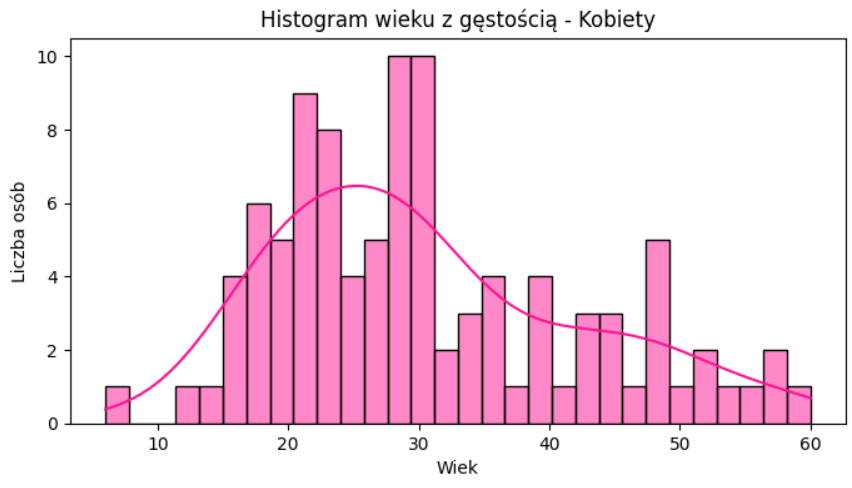
\includegraphics[width=0.9\textwidth]{Histogram_Kobiety.png}
	\end{figure}
	\begin{figure}[h]
		\centering
		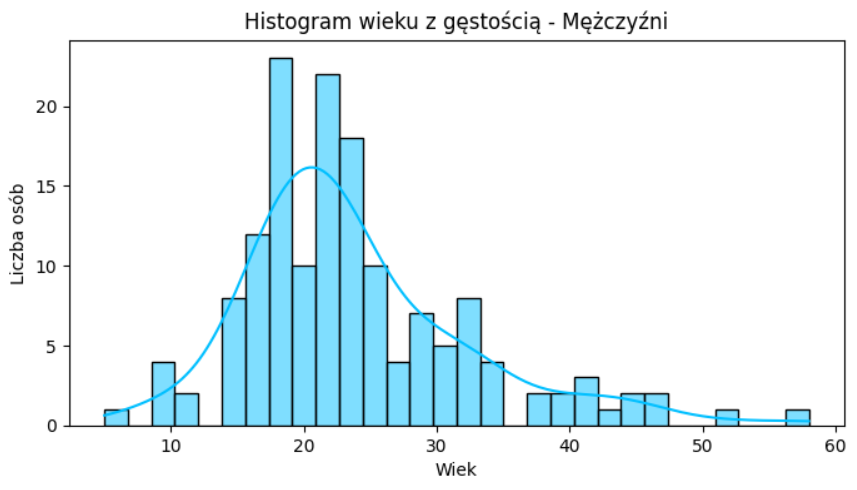
\includegraphics[width=0.9\textwidth]{Histogram_m.png}
	\end{figure} \\
	\newpage
	\noindent
	\textbf{Kobiety:}
	\begin{itemize}
		\item Histogram przedstawia rozkład wieku kobiet w próbie.
		\item Kształt rozkładu wydaje się zbliżony do normalnego, jednak może być lekko asymetryczny w prawo (prawostronnie skośny) co sugeruje dłuższy ogon po stronie wyższych wartości wieku.
		\item Obserwujemy, że większość kobiet znajduje się w przedziale ok. 20-35 lat, co może wskazywać na specyficzną charakterystykę badanej populacji (np. młode dorosłe).
		\item Estymowana gęstość (KDE) jest gładka i jednolita, bez wielomodalnych pików, co oznacza brak wyraźnych podgrup wiekowych.
	\end{itemize}
	\textbf{Mężczyźni:}
	\begin{itemize}
		\item Wiek mężczyzn również koncentruje się w przedziale ok. 20-35 lat, ale rozkład jest nieco bardziej rozciągnięty w porównaniu do kobiet.
		\item Krzywa KDE pokazuje możliwe delikatne spłaszczenie szczytu, co może sugerować większe zróżnicowanie wśród mężczyzn niż kobiet.
		\item Brak ostrych pików wskazuje na brak wyraźnych skoków w częstości, co świadczy o płynnym rozkładzie danych.
		\item Możemy tutaj zaobserwować wartości odstające.
	\end{itemize}
	\textbf{Wnioski:}
	\begin{itemize}
		\item Dla obu grup rozkład wieku jest stosunkowo symetryczny, co jest dobrą przesłanką do stosowania metod opartych na założeniu normalności.
		\item Różnice między płciami są niewielkie, choć możliwe jest nieco większe zróżnicowanie weku w grupie mężczyzn.
	\end{itemize}
	\subsection{Analiza dystrybuanty wieku}
	\noindent
	Aby dokładniej ocenić rozkład wieku w badanej grupie pacjentów, przeprowadzimy analizę empirycznych dystrybuant rozkłady (ECDF) osobno dla kobiet i mężczyzn. Dystrybuanta empiryczna pozwala zobrazować, jak rozkładają się wartości zmiennej losowej w próbie i jest szczególnie przydatna przy porównywaniu z modelem teoretycznym. W analizie uwzględniono również teoretyczną dystrybuantę rozkładu normalnego dopasowaną do danych, w celu oceny zgodności empirycznego rozkładu z rozkładem normalnym. Takie porównanie umożliwia wizualne wykrycie ewentualnych odchyleń, takich jak skośność, czy obecność wartości odstających, które mogą wpływać na dobór odpowiednich metod statystycznych w dalszych etapach analizy.
	\begin{figure}[h]
		\centering
		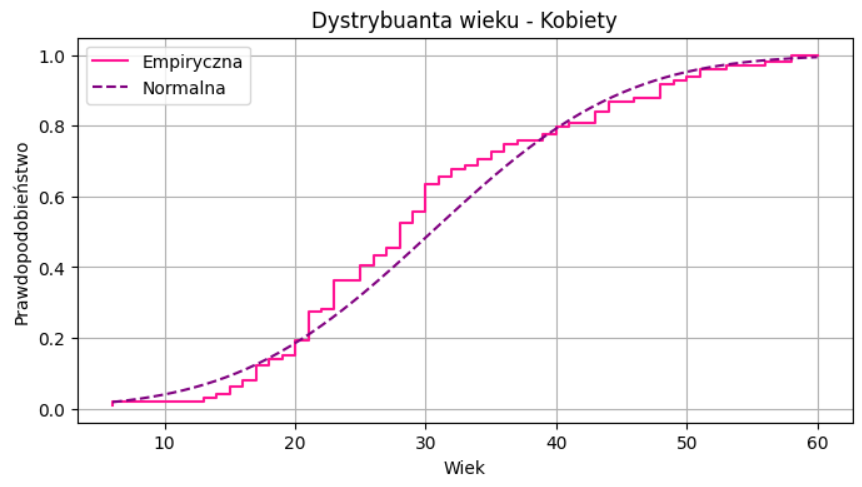
\includegraphics[width=0.9\textwidth]{Dys_k.png}
	\end{figure}
	\begin{figure}[h]
		\centering
		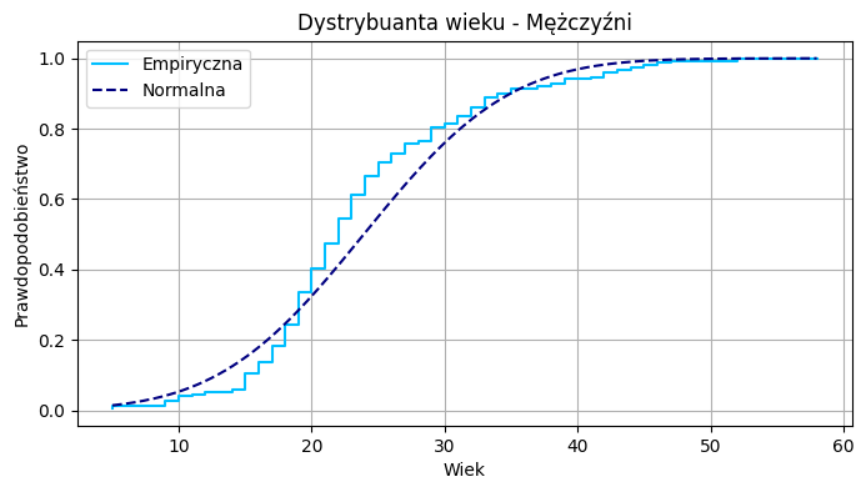
\includegraphics[width=0.9\textwidth]{Dyst_m.png}
	\end{figure} 
	\newpage
	\noindent
	\textbf{Kobiety:} \\
	Na pierwszym wykresie przedstawiono empiryczną dystrybuantę wieku kobiet zestawioną z teoretyczną dystrybuantą rozkładu normalnego. Obserwujemy, że:
	\begin{itemize}
		\item W środkowym zakresie wartości (ok. 25-40 lat) przebieg ECDF jest bardzo zbliżony do teoretycznej krzywej, co sugeruje dobrą zgodność z rozkładem normalnym.
		\item Na krańcach (poniżej 20 i powyżej 45 roku życia) widoczne są niewielkie odchylenia - empiryczna krzywa rośnie nieco wolniej nż normalna, co może oznaczać nieco spłaszczony rozkład.
		\item Nie obserwowano gwałtownych soków ani długich ogonów, co potwierdza brak istotnych wartości odstających.
	\end{itemize}
	Wiek kobiet można traktować jako rozkładający się blisko normalności, z lekkimi odchyleniami na obrzeżach rozkładu. \\
	\textbf{Mężczyźni:} \\
	Na drugim wykresie przedstawiono analogiczną analizę dla mężczyzn. Empiryczna dystrybuanta przebiega mniej regularnie i w kilku miejscach wyraźnie odchyla się od dystrybuanty normalnej.
	\begin{itemize}
		\item W środkowym zakresie dopasowanie jest dobre, natomiast w okolicach 25-50 lat obserwuje się znacznie wolniejszy przyrost ECDF, co świadczy o obecności większej liczby starszych pacjentów niż przewidywałby rozkład normalny.
		\item Takie zachowanie wskazuje na prawoskośność rozkładu - potwierdzaną również przez wcześniejsze wykrycie wartości odstających.
		\item Możliwe także, że dane są lekko zanieczyszczone szumem.
	\end{itemize}
	Wiek mężczyzn odbiega od rozkładu normalnego bardziej niż w przypadku kobiet.
	\subsection{Analiza wieku za pomocą wykresu pudełkowego}
	\noindent
	Na poniższym wykresie przedstawiono porównanie rozkładów wielu kobiet i mężczyzn z wykorzystaniem wykresu pudełkowego. Metoda ta umożliwia szybkie rozpoznanie mediany, rozrzutu, asymetrii oraz obecności wartości odstających w danych.
	\newpage
	\begin{figure}[h]
		\centering
		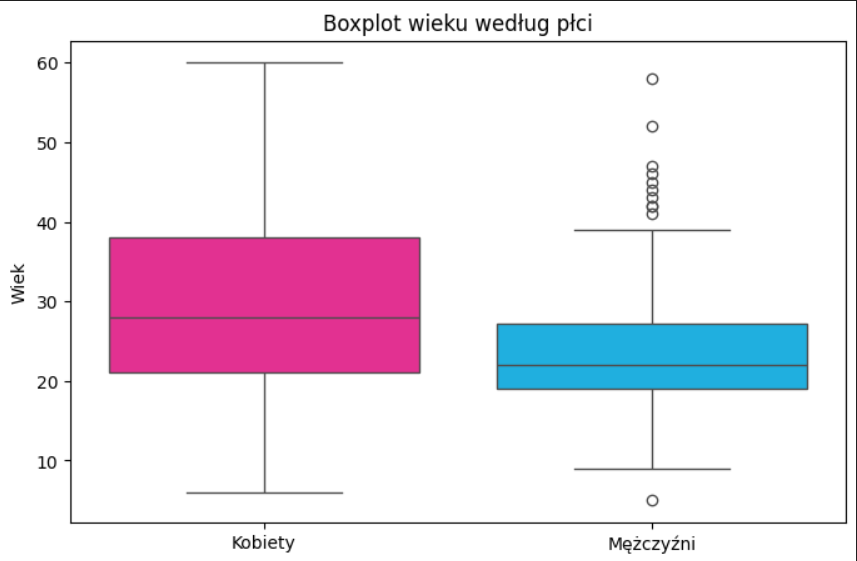
\includegraphics[width=0.9\textwidth]{Box.png}
	\end{figure} 
	\noindent
	\textbf{Kobiety:}
	\begin{itemize} 
		\item Mediana wieku wynosi około 28 lat, co wskazuje, że połowa badanych kobiet ma mniej niż 28 lat, a połowa więcej.
		\item  Rozstęp między kwartylowy (IQR), czyli zakres między pierwszym a trzecim kwartylem, jest stosunkowo szeroki, co świadczy o znacznej zmienności wieku w tej grupie.
		\item Brak wartości odstających (żadnych punktów poza wąsami), co oznacza, że dane kobiet są bardziej jednorodne i symetryczne.
		\item Wąsy wykresu rozciągają się od ok. 6 do 60 lat, co odpowiada pełnemu zakresowi obserwowanych wartości.
	\end{itemize}
	Rozkład wieku kobiet jest szeroki, ale pozbawiony skrajnych wartości. Brak wartości odstających potwierdza stabilność próbki i zgodność z rozkładem normalnym. \\
	\textbf{Mężczyźni:} 
	\begin{itemize}
		\item Mediana wieku mężczyzn to około 22 lata, czyli zauważalnie niższa niż u kobiet.
		\item Rozstęp między kwartylowy jest mniejszy niż u kobiet, co sugeruje mniejszą zmienność wieku w tej grupie.
		\item Obserwuje się liczne wartości odstające, oznaczone jak pojedyncze punkty - głównie w przedziale powyżej 40 lat.
		\item Dolna granica sięga 8 lat, natomiast górna kończy się na koło 40 latach, co wskazuje na silne zgrupowanie danych w młodszych przedziałach wiekowych.
	\end{itemize}
	Grupa mężczyzn charakteryzuje się niższą medianą i większą koncentracją wieku wokół młodszych wartości. Jednocześnie liczne wartości odstające wskazują na obecność starszych pacjentów, co wpływa na asymetrię i może zaburzać analizę rozkładu.
	\subsection{Analiza QQ-plotów}
	\noindent
	QQ-ploty służą do wizualnej oceny zgodności rozkładu danych empirycznych z rozkładem normalnym. Porównują one kwantyle danych z kwantylami teoretycznego rozkładu normalnego, jeżeli dane pochodzą z rozkładu normalnego, punkty na wykresie powinny układać się wzdłuż linii prostej.
	\newpage
	\begin{center}
		\begin{minipage}{0.9\textwidth}
			\centering
			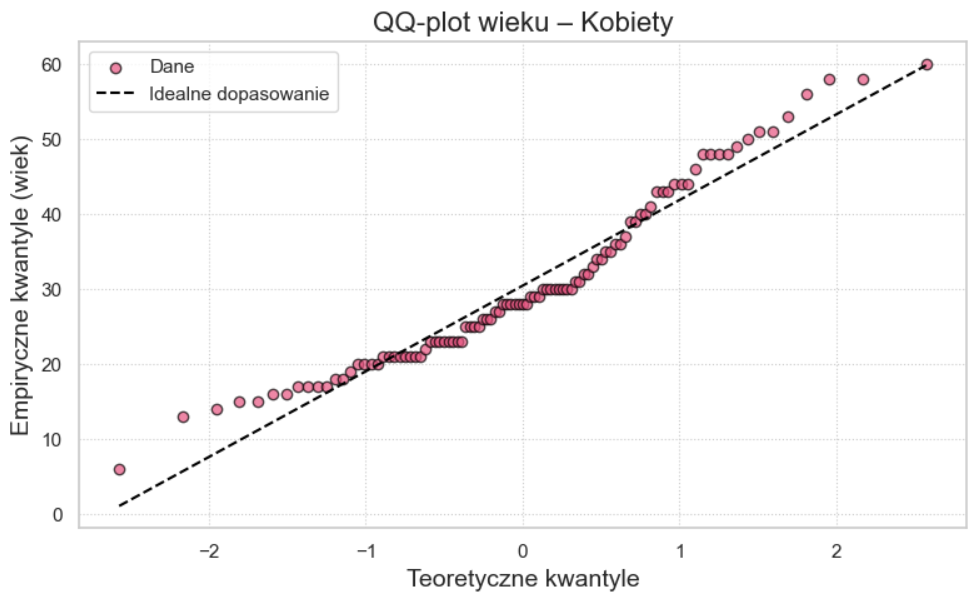
\includegraphics[width=\textwidth]{qq_k.png}
		\end{minipage}
		
		\vspace{1em} 
		
		\begin{minipage}{0.9\textwidth}
			\centering
			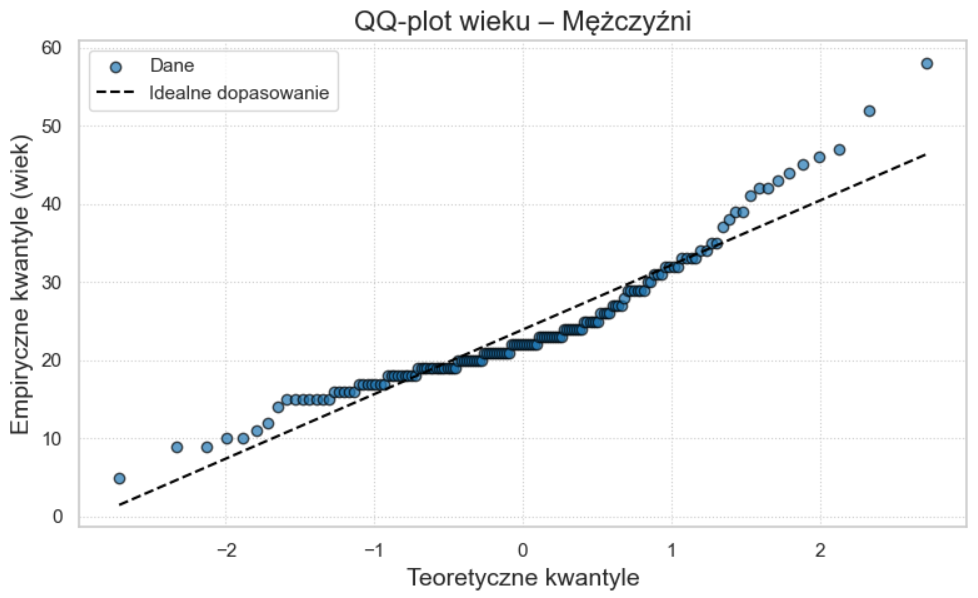
\includegraphics[width=\textwidth]{qq_m.png}
		\end{minipage}
	\end{center}
	\noindent
	\textbf{Kobiety:}
	\begin{itemize}
		\item Punkty na QQ-plocie dla kobiet układają się blisko linii przekątnej, co sugeruje, że rozkład wieku w tej grupie jest zbliżony do normalnego.
		\item Niewielkie odchylenia na krańcach (tzw. ogonach) są naturalne i nie wskazują na istotne odstępstwa.
		\item Brak widocznych wartości odstających oraz równomierne rozmieszczenie punktów potwierdzają symetrię rozkładu i jego zgodność z rozkładem normalnym.
	\end{itemize}
	\noindent
	\textbf{Mężczyźni:}
	\begin{itemize}
		\item QQ-plot dla mężczyzn wykazuje zauważalne odchylenia od linii prostej, szczególnie dla wyższych wartości wieku.
		\item W prawej części wykresu punkty wyraźnie przekraczają linię oczekiwaną, co wskazuje na obecność dłuższego prawego ogona, która jest typową cechę prawostronnej skośności.
		\item Takie zachowanie koreluje z obserwowanymi wartościami odstającymi oraz większym rozrzutem, zaobserwowanymi wcześniej na histogramie i wykresie pudełkowym.
	\end{itemize}
	$\,$\\
	\textbf{Wnioski z QQ-plotów:}
	\begin{itemize}
		\item Rozkład wieku kobiet można uznać za zgodny z rozkładem normalnym, co umożliwia stosowanie klasycznych metod parametrycznych.
		\item W przypadku mężczyzn rozkład wieku odbiega od normalności, co sugeruje rozważenie alternatywnych metod nieparametrycznych (np. test U Manna-Whitneya).
	\end{itemize}
	
	\section{Podsumowanie}
	\noindent
	Analiza statystyczna wieku zachorowania na schizofrenię ujawniła wyraźne różnice między kobietami a mężczyznami. Kobiety chorują średnio później (średnia wieku: 30{,}47 lat) niż mężczyźni (23{,}91 lat), co potwierdzają zarówno klasyczne, jak i odporne na wartości odstające miary tendencji centralnej (średnia, mediana, kwartyle).\\
	\noindent 
	Rozproszenie wieku zachorowania jest większe wśród kobiet – ich dane wykazują większą wariancję, szerszy rozstęp międzykwartylowy (IQR) oraz wyższe odchylenie standardowe. Mężczyźni cechują się bardziej skupionym rozkładem wieku, ale z wyraźnie zaznaczoną prawostronną skośnością oraz obecnością licznych wartości odstających, co potwierdzają QQ-ploty i wykresy pudełkowe.\\
	\noindent
	Rozkład wieku kobiet jest bliższy normalnemu – symetryczny, jednorodny i pozbawiony skrajnych wartości – co umożliwia stosowanie metod parametrycznych. U mężczyzn rozkład jest asymetryczny i bardziej zróżnicowany na krańcach, co przemawia za użyciem metod nieparametrycznych w dalszych analizach.\\
	\noindent
	\textbf{Wniosek ogólny:} Kobiety zapadają na schizofrenię istotnie później i w bardziej zróżnicowanym wieku niż mężczyźni, u których choroba występuje wcześniej, lecz z większym udziałem wartości odstających. Te różnice mają znaczenie praktyczne przy doborze metod analizy statystycznej i mogą wpływać na strategie diagnozowania i leczenia.
	
	
	
	
\end{document}